\documentclass[../main.tex]{subfiles}
\begin{document}
\subsubsection{Critical slowing down as loss of resilience}\label{subsubsec1.2.1}
Detection of early signs of incoming catastrophic events can take several forms. As mentioned above, the first occurence that was proposed as a precursor of such events is a phenomenon known as CSD.
The origin of the adoption of this term in dynamical systems can be traced back to 1994 Strogatz's seminal book \cite{Strogatz94} (which further mentions the name to be coined in statistical mechanics) and it referred to the lethargic (algebraic) decay of solutions to the stable equilibrium in the proximity of a supercritical pitchfork bifurcation (as opposed to the fast, exponential decay away from the bifurcation). 
\paragraph{1980s and 1990s}
This was proved mathematically one decade earlier in \cite{Wissel84} where it was shown how the return time of the system to its attractor depends on the inverse of the leading eigenvalue of the linearisation of the dynamics around the equilibrium.
As such attractor approaches a critical threshold it would thus exhibit infinitely slower return rate from a small perturbation.
As far as we know, the characteristic return time is the first indicator foretelling a critical transition.
The derivation of this \textit{``universal law"} was motivated by the study of thresholds of instabilities in multi-stable ecological systems \cite{May77} which in retrospective appears to be somehow prophetic of the communities that will extensively apply CSD forewarning catastrophic population collapses 2 decades later.
The influence of noise in such perturbations was characterised shortly thereafter in \cite{Wiesenfeld86} which linked the frequency range of the disturbance with the simplest codim$-1$ bifurcations showing that small-signal amplification was indeed a feature of these autonomous dynamical systems.
In 1995 this concept was (arguably independently) explored in \cite{Ives95} for stochastic dynamical systems. 
In there the \textit{resilience} of ecological systems was quantified statistically to be the ratio of the variability of population densities to variability in population growth rates. The study mentions the return time to equilibrium as the deterministic equivalent of stochastic resilience.
\begin{figure}[H]
    \centering 
    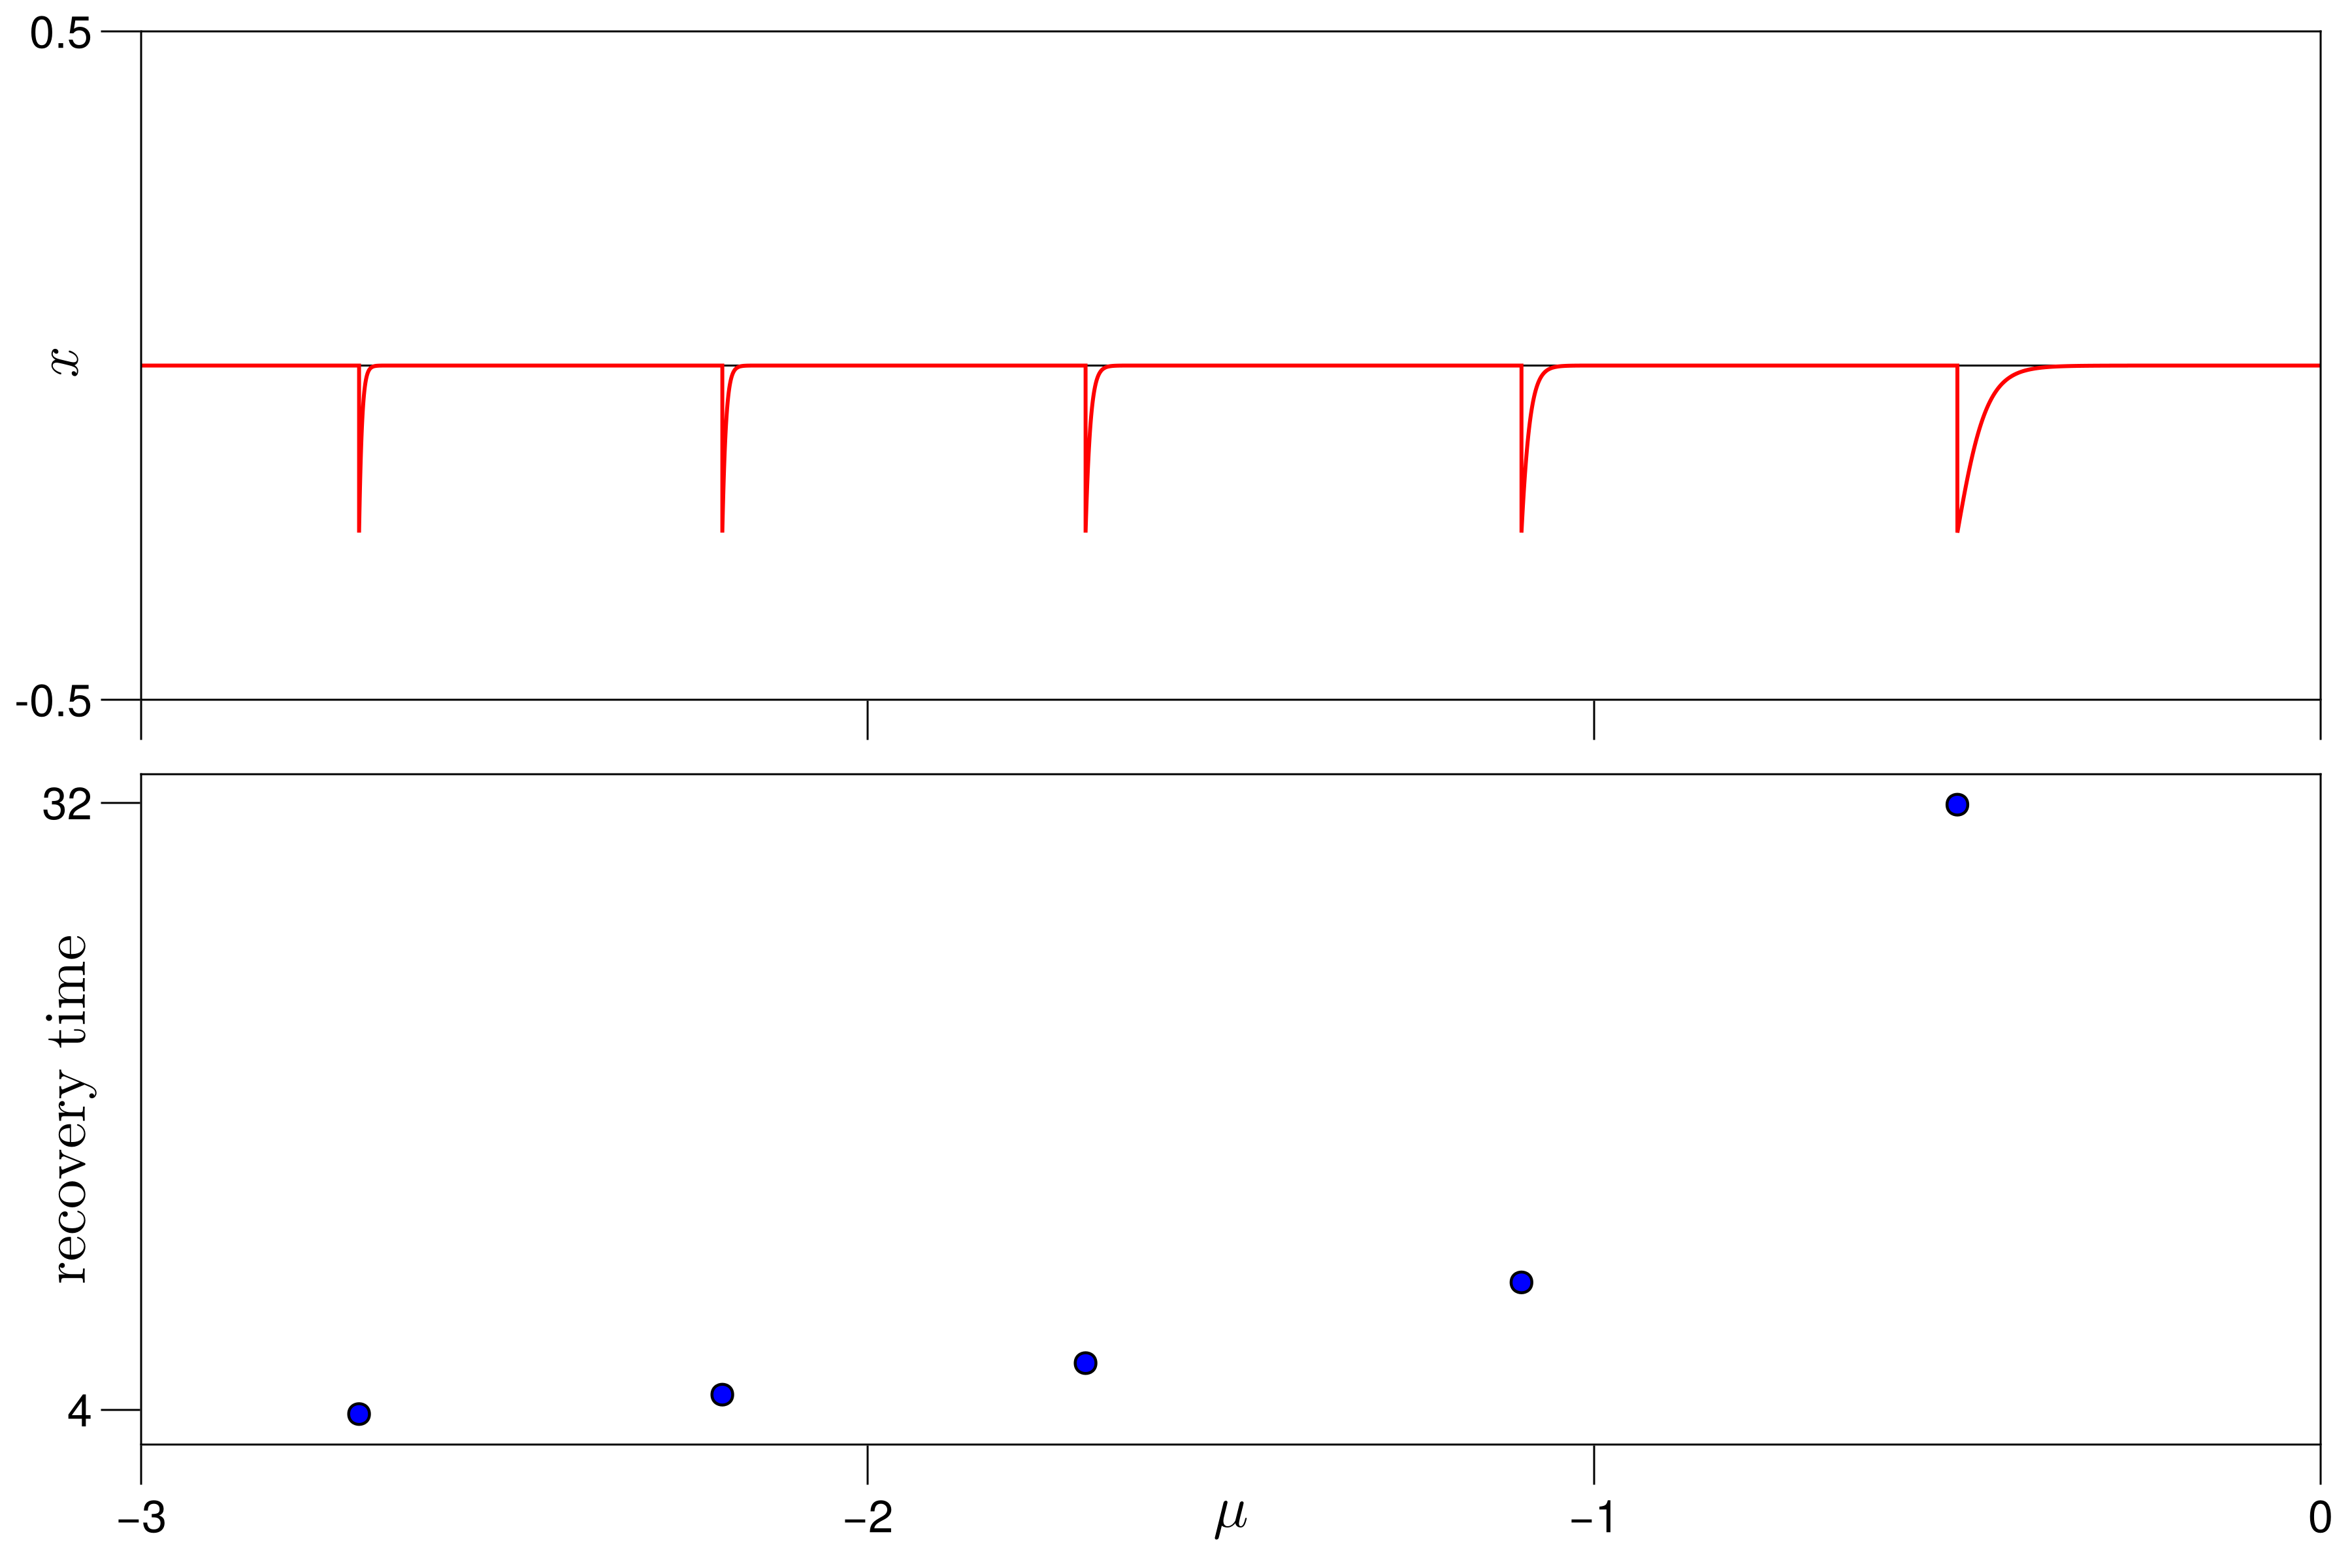
\includegraphics[keepaspectratio, width=\textwidth]{../figures/fig1.2.png}
    \caption{The phenomenon of CSD illustrated for a transcritical normal form. As the parameter approaches the bifurcation value $\mu=0$ small perturbations of the state (red line) tracking the attractor $x=0$ result in increasingly longer recovery. The return time is estimated numerically (blue dots) for each perturbation.}
    \label{fig1.2}
\end{figure}
It then took almost one decade to the ecologists to realise that, as catastrophic switches between stable population's states occurred unannounced when one only monitors the state variables (as for a saddle-node bifurcation \cite{Scheffer01}) the derivation of EWS was necessary to predict these disruptive shifts and act upon the external forcing to prevent them. 
\paragraph{Mid 2000s}
In 2005 it was observed \cite{Oborny05} that the spatial dynamics of a logistic model organised on a square lattice exhibits fractal-like subdivisions of the competing species and suggested that the scaling law of the spatial variance near the extinction can be used as a EWS. 
It was one year later when Carpenter and Brock \cite{Carpenter06} formalised this idea and conjectured how increases in the variance of the timeseries of a stochastic differential equation (SDE) can be a clue of impending regime shifts.
The rise in variance of SDEs as an indicator of CSD will not be rigorously proved mathematically for another 5 years when Kuehn \cite{Kuehn11} formalised it in the framework of fast-slow dynamics (discussed later in Section \ref{subsubsec2.1.3}).
Nevertheless there is a pleasant intuition for this measure of CSD as discussed in \cite{Scheffer09}. 
As CSD is associated to a slower recovery from forced perturbations, due to the leading eigenvalue of the respective Jacobian approaching the immaginary axis, the intrinsic rate of change of the realizations of the SDE diminishes. 
This in turn is reflected in the timeseries to exhibit memory of its past i.e. the state at the next iteration will be somewhat related to some order of its past states. 
This intuition is already enough to suggest the autocorrelation of lagging order $p$ (AC($p$)) to be an indicator of CSD.
However if one is willing to force some form of equivalence between a more sluggish timeseries w.r.t. perturbations and a random walk (which has a monotonic trend in variance depending linearly on time) then rise in the variance can be reasonably assumed as an EWS of an upcoming bifurcation.
Perhaps the major significance of Carpenter's and Brock's 2006 paper for the ecology community was the suggested implication that, by relying merely on timeseries data, a catastrophic population collapse can be predicted early enough even without knowing the underlying model (or assuming high levels of uncertainties in the estimation of parameters and noise levels). 
Prior to their proposal however, earlier works in the climate community proposed different types of indicators for estimating the distance to bifurcations of the North Atlantic thermoaline circulation (THC) under (stochastic) freshwater forcing driven by climate change. 
In particular in 2003 a simplified box model of the THC was deployed to estimate (analytically) the dependence of shifts in the frequency spectrum of the idealised Ornstein-Uhlenbeck process (OUP) of the deviations of the salinity gradient from equilibrium to the (bi-stable) saddle-node bifurcation in the model \cite{Kleinen03} (which became known as spectral reddening).
One year later the same first author also co-authored an investigation for larger, more realistic models of the THC in a numerical setting \cite{Held04} and concluded that an increased variability is a better diagnostic tool at anticipating the overturning circulation.
These works spurred a vast uptake by climate scientist and ecologist in the role of CSD and in general in the potential of statistical measures that are prognostics of catastrophic regime shifts in their respective systems.
\end{document}
